%--------------------------------------------------------------------------------------------------------------
% kapitel/grundlagen.tex
%--------------------------------------------------------------------------------------------------------------

\chapter{Theoretische Grundlagen}

In diesem Kapitel werden zunächst die Grundlagen und Begrifflichkeiten vorgestellt. Weiterhin werden die Kriterien für eine erfolgreiche Migrationen erläutert.

\section{SIV.AG}\label{SIV.AG}

Die SIV.AG ist ein Anbieter für ganzheitliche Lösungen im Bereich der deutschen und internationalen Energie- und Wasserwirtschaft. Das Kernstück vom Unternehmen ist das Softwareprodukt kVASy$^\text{\textregistered}$, ein vollständig integriertes \acrfull{erp}, welches insbesondere auf die Anforderungen und Prozesse der Energie- und Wasserwirtschaft ausgerichtet ist. Das Unternehmen wurde 1990 durch Jörg Sinnig als Software- und Beratungshaus gegründet. Zum gegenwärtigen Zeitpunkt beschäftigt die SIV.AG mehr als 400 Mitarbeiter. Ihr Leistungsportfolio reicht von der Beratung und Analyse über die Implementierung und Bereitstellung der IT-Systeme bis hin zur Datenmigration, Schulung und Pflege.\cite{SIV13}

\section{kVASy\texorpdfstring$^\text{\textregistered}$}

Das zuvor bereits erwähnte kVASy$^\text{\textregistered}$ ist ein webbasiertes \acrshort{erp} und bildet das Aushängeschild der SIV.AG. Zu der Produktfamilie gehören die 4 Bereiche Finance (Buchaltung), Billing (Abrechnung) und EDM (Vertragsverwaltung), Technical Assets (Anlagenmanagement) und xRM (Kundenbeziehungsmanagement).

\section{Datenbanksysteme}
\subsection{Elemente eines relationalen Datenbanksystems}
\subsection{Beziehungen und Normalformen}
\subsection{Schema}

\section{Datenintegration/Datenmigration}

\section{Transformationen}

\section{ETL-Tools}

\section{Qualitätskontrolle/Protokollierung}

\section{Kriterien für erfolgreiche Migrationen}
\begin{itemize}

  \item Ziele einer Migration
  \item Vorgehensweise/Migrationsplanung
  \item Strategische Aspekte
  \item Rechtliche Aspekte
  \item Wirtschaftliche Aspekte
  \item Qualitative Aspekte
  \item Aspekte des Systembetriebs
  \item Organisatorische Aspekte
  \item Sicherheitsaspekte
\end{itemize}
\subsection{Ziele einer Migration}
Bevor es zur einer 
\begin{itemize}
  \item ein verbesserter Anwendernutzen
  \item das Herstellen eines rechtlich notwendigen Zustands
  \item die Behebung von Fehlern
  \item die Erweiterung des Funktionsumfangs
  \item eine verbesserte Integration in die vorhandenen Softwaresysteme
  \item eine verbesserte Interoperabilität
  \item eine Verringerung der laufenden Kosten
  \item die Erhöhung der Produktivität
  \item die bessere Nutzung vorhandener Resourcen
  \item die Einhaltung strategischer Vorgaben
\end{itemize}
\subsection{Wirtschaftliche Aspekte}
\subsection{Qualitative Aspekte}
\subsection{Organisatorische Aspekte}
\subsection{Vorgehensweise/Migrationsplanung}
\subsection{Anforderung an die Datenmigration}


% \subsection{Bilder}
% Beispiel für ein Bild in \LaTeX{}
% \begin{figure}[ht]
% 	\begin{center}
% 		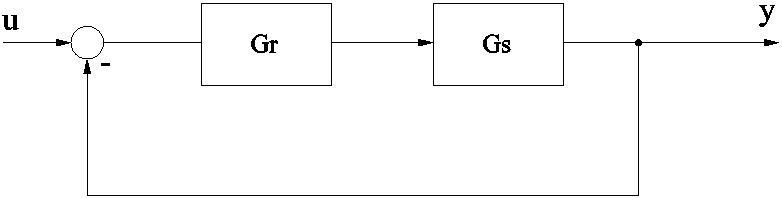
\includegraphics[scale=0.3]{bilder/regelkreis.png}
% 		\caption{Ein Standard-Regelkreis}
% 		\label{pic:grund:regelkreis}
% 	\end{center}
% \end{figure}

% \subsection{Tabellen}
% Beispiel für eine Tabelle in \LaTeX{}
% \begin{table}[ht]
% 	\begin{center}
% 		\caption{Verwendete Matrizen}
% 		\begin{tabular}{|l|l|l|}
% 			\hline
% 			Matrix& Dimension& Symbol\\
% 			\hline
% 			Systemmatrix& $n\times n$& \textrm{A}\\
% 			\hline
% 			Ausgangsmatrix& $m\times n$& \textrm{C}\\
% 			\hline
% 		\end{tabular}
% 		\label{tab:grund:matrizen}
% 	\end{center}
% \end{table}
% 
% \subsection{Formeln}
% Beispiel für eine Formel in \LaTeX{}
% \begin{equation}
% 	c^2 = a^2 + b^2
% \end{equation}
% und noch eine Formel
% \begin{equation}
% 	f_1(x) = x_1 + x_2 + x_3
% \end{equation}
% Für weitere Möglichkeiten Formeln in \LaTeX{} einzufügen, schauen sie bitte in \cite{Peters2005}.
% 
% \subsection{{Bib\TeX}}
% Bib\TeX{} ermöglicht das erstellen eines Literaturverzeichnisses. Für die die sich weiter einarbeiten wollen, empfehle ich folgende Seite \cite{wiki:bibtex}.
% 
% \subsection{Abkürzungen}
% Es wird das Package \textit{glossary} verwendet. Mit ihm ist es möglich ein Abkürzungsverzeichnis und ein Glossary zu erstellen. Beispiel: \acrfull{lan} \acrfull{www}
